%!TEX program = xelatex+makeindex+bibtex
\documentclass[final]{scrreprt} %scrreprt of scrartcl
\usepackage{amsmath}
% Include all project wide packages here.
\usepackage{fullpage}
\usepackage{polyglossia}
\setmainlanguage{english}
\usepackage{csquotes}
\usepackage{graphicx}
\usepackage{epstopdf}
\usepackage{pdfpages}
\usepackage{caption}
\usepackage[list=true]{subcaption}
\usepackage{float}
\usepackage{standalone}
\usepackage{import}
\usepackage{tocloft}
\usepackage{wrapfig}
\usepackage{authblk}
\usepackage{array}
\usepackage{booktabs}
\usepackage[toc,page,title,titletoc]{appendix}
\usepackage{xunicode}
\usepackage{fontspec}
\usepackage{pgfplots}
\usepackage{SIunits}
\usepackage{units}
\pgfplotsset{compat=newest}
\pgfplotsset{plot coordinates/math parser=false}
\newlength\figureheight 
\newlength\figurewidth
\usepackage{amsmath}
\usepackage{mathtools}
\usepackage{unicode-math}
\usepackage[
    backend=bibtexu,
	texencoding=utf8,
bibencoding=utf8,
    style=ieee,
    sortlocale=en_US,
    language=auto
]{biblatex}
\usepackage{listings}
\newcommand{\includecode}[3][c]{\lstinputlisting[caption=#2, escapechar=, style=#1]{#3}}
\newcommand{\superscript}[1]{\ensuremath{^{\textrm{#1}}}}
\newcommand{\subscript}[1]{\ensuremath{_{\textrm{#1}}}}


\newcommand{\chapternumber}{\thechapter}
\renewcommand{\appendixname}{Bijlage}
\renewcommand{\appendixtocname}{Bijlagen}
\renewcommand{\appendixpagename}{Bijlagen}

\usepackage[hidelinks]{hyperref} %<--------ALTIJD ALS LAATSTE

\renewcommand{\familydefault}{\sfdefault}

\setmainfont[Ligatures=TeX]{Myriad Pro}
\setmathfont{Asana Math}
\setmonofont{Lucida Console}

\usepackage{titlesec, blindtext, color}
\definecolor{gray75}{gray}{0.75}
\newcommand{\hsp}{\hspace{20pt}}
\titleformat{\chapter}[hang]{\Huge\bfseries}{\chapternumber\hsp\textcolor{gray75}{|}\hsp}{0pt}{\Huge\bfseries}
\renewcommand{\familydefault}{\sfdefault}
\renewcommand{\arraystretch}{1.2}
\setlength\parindent{0pt}

%For code listings
\definecolor{black}{rgb}{0,0,0}
\definecolor{browntags}{rgb}{0.65,0.1,0.1}
\definecolor{bluestrings}{rgb}{0,0,1}
\definecolor{graycomments}{rgb}{0.4,0.4,0.4}
\definecolor{redkeywords}{rgb}{1,0,0}
\definecolor{bluekeywords}{rgb}{0.13,0.13,0.8}
\definecolor{greencomments}{rgb}{0,0.5,0}
\definecolor{redstrings}{rgb}{0.9,0,0}
\definecolor{purpleidentifiers}{rgb}{0.01,0,0.01}


\lstdefinestyle{csharp}{
language=[Sharp]C,
showspaces=false,
showtabs=false,
breaklines=true,
showstringspaces=false,
breakatwhitespace=true,
escapeinside={(*@}{@*)},
columns=fullflexible,
commentstyle=\color{greencomments},
keywordstyle=\color{bluekeywords}\bfseries,
stringstyle=\color{redstrings},
identifierstyle=\color{purpleidentifiers},
basicstyle=\ttfamily\small}

\lstdefinestyle{c}{
language=C,
showspaces=false,
showtabs=false,
breaklines=true,
showstringspaces=false,
breakatwhitespace=true,
escapeinside={(*@}{@*)},
columns=fullflexible,
commentstyle=\color{greencomments},
keywordstyle=\color{bluekeywords}\bfseries,
stringstyle=\color{redstrings},
identifierstyle=\color{purpleidentifiers},
}

\lstdefinestyle{matlab}{
language=Matlab,
showspaces=false,
showtabs=false,
breaklines=true,
showstringspaces=false,
breakatwhitespace=true,
escapeinside={(*@}{@*)},
columns=fullflexible,
commentstyle=\color{greencomments},
keywordstyle=\color{bluekeywords}\bfseries,
stringstyle=\color{redstrings},
identifierstyle=\color{purpleidentifiers}
}

\lstdefinestyle{vhdl}{
language=VHDL,
showspaces=false,
showtabs=false,
breaklines=true,
showstringspaces=false,
breakatwhitespace=true,
escapeinside={(*@}{@*)},
columns=fullflexible,
commentstyle=\color{greencomments},
keywordstyle=\color{bluekeywords}\bfseries,
stringstyle=\color{redstrings},
identifierstyle=\color{purpleidentifiers}
}

\lstdefinestyle{xaml}{
language=XML,
showspaces=false,
showtabs=false,
breaklines=true,
showstringspaces=false,
breakatwhitespace=true,
escapeinside={(*@}{@*)},
columns=fullflexible,
commentstyle=\color{greencomments},
keywordstyle=\color{redkeywords},
stringstyle=\color{bluestrings},
tagstyle=\color{browntags},
morestring=[b]",
  morecomment=[s]{<?}{?>},
  morekeywords={xmlns,version,typex:AsyncRecords,x:Arguments,x:Boolean,x:Byte,x:Char,x:Class,x:ClassAttributes,x:ClassModifier,x:Code,x:ConnectionId,x:Decimal,x:Double,x:FactoryMethod,x:FieldModifier,x:Int16,x:Int32,x:Int64,x:Key,x:Members,x:Name,x:Object,x:Property,x:Shared,x:Single,x:String,x:Subclass,x:SynchronousMode,x:TimeSpan,x:TypeArguments,x:Uid,x:Uri,x:XData,Grid.Column,Grid.ColumnSpan,Click,ClipToBounds,Content,DropDownOpened,FontSize,Foreground,Header,Height,HorizontalAlignment,HorizontalContentAlignment,IsCancel,IsDefault,IsEnabled,IsSelected,Margin,MinHeight,MinWidth,Padding,SnapsToDevicePixels,Target,TextWrapping,Title,VerticalAlignment,VerticalContentAlignment,Width,WindowStartupLocation,Binding,Mode,OneWay,xmlns:x}
}

%defaults
\lstset{
basicstyle=\ttfamily\small,
extendedchars=false,
numbers=left,
numberstyle=\ttfamily\tiny,
stepnumber=1,
tabsize=4,
numbersep=5pt
}
\addbibresource{../../library/bibliography.bib}

\begin{document}

\chapter{Wireless charging}
In order to wirelessly charge KITT we had to design a DC-DC converter. The DC-DC converter is splitted into two parts, the DC-AC converter and AC-DC converter respectively. 
For the DC-AC converter see Figure \ref{fig:DC-AC} and for the AC-DC see Figure \ref{fig:AC-DC}

\begin{figure}[h]
	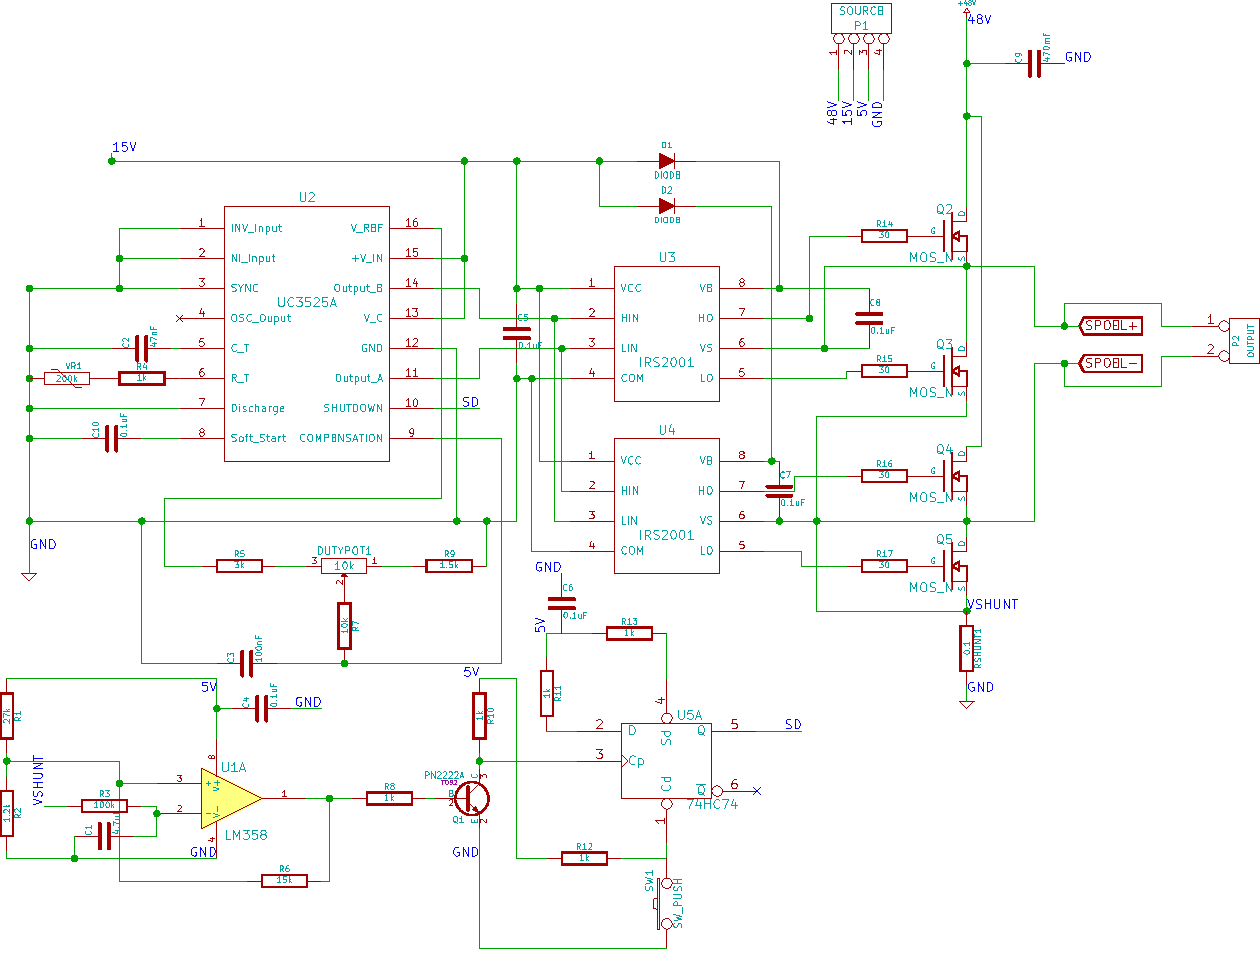
\includegraphics[width=\linewidth]{resources/DC-AC-rc.pdf}
	\caption{DC-AC subcircuit}
	\label{fig:DC-AC}
\end{figure}

\begin{figure}[h]
	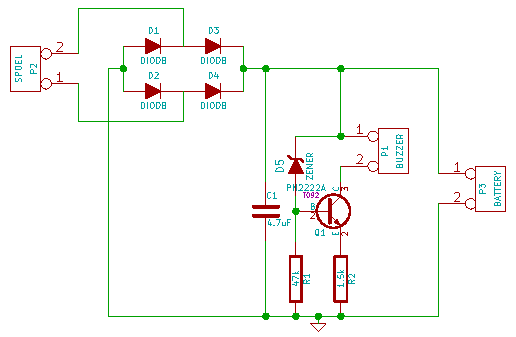
\includegraphics[width=\linewidth]{resources/AC-DC-rc.pdf}
	\caption{AC-DC subcircuit}
	\label{fig:AC-DC}
\end{figure}

For the NMOS transistor used in Figure \ref{fig:DC-AC} we used the IPP028N08N3G (OptiMOS 3) transistor instead of the IPP50CN10N (OptiMOS 2).
We had two reasons for this decision.
\begin{enumerate}
\item First, the drain-source on-state resistance was approximately ten times lower on the OptiMOS 3, causing the transistor to generate less heat and gain better efficiency.
\item Secondly, by looking at the current-voltage characteristics per frequency (\cite{OptiMOS2} \emph{:3 Safe operating area} and \cite{OptiMOS3} \emph{:3 Safe operating area}) we found out that the OptiMOS 3 performs better at higher frequencies than the OptiMOS 2.
\end{enumerate}

We also had to choose the diodes used on the secondary side of the tranformer. 
The diodes will form a full bridge rectifier, which, in combination with a capacitor, will form a AC-DC converter.
The candidates are the SB540 (datasheet: \cite{SB540}) and the SF61 (datasheet: \cite{SF61}).
The forward voltage of the two diodes differ, the SB540's is lower. 
This is favorable since there will be more voltage left on the output terminals.
On the other hand, the SF61 has a much lower reverse current. 
Lower reverse current makes the diode more ideal, since it should only conduct when the current is in forward direction.
The SB530 would be the better option when weighting these pros and cons since the reverse current is small enough with both diodes, but the forward voltage makes a rather large difference.
However, we did not implement these diodes because we did not know the forward voltage was more important at that time.
In the near future, we might replace the diodes with the SB540 to gain a better performance. \\




The next step in designing our DC-DC converter was to design the air-coupled transformer. 
In order to find how many windings we need per coil we used \cite{windings}.
Through this site we found that we needed 40 windings for our primary coil of roughly \unit{200}{\micro}H and 14.44 windings for our secondary coil of roughly \unit{20}{\micro}H.
The mutual inductance of the two coils can be found by measuring both the opposing and aiding configuration of the coils. 
The results for these measurements are given in Table \ref{tab:inductances}.

\begin{table} [h]
\begin{center}
	\begin{tabular}{ l | l | l | l | l }
	Distance & Aiding inductance ($\mu$H) & Opposing inductance ($\mu$H) & Mutual inductance ($\mu$H) & k \\ \hline
  	0 cm & 312.5 & 145.8 & 41.7 & 0.599 \\
	2 cm & 276.0 & 186.4 & 22.4 & 0.322 \\
	4 cm & 258.0 & 199.3 & 14.7 & 0.211 \\
	6 cm & 248.0 & 204.0 & 11.0 & 0.158 \\
	\end{tabular}
	\caption{Inductance in aiding and opposing configuration plus conclusion}
	\label{tab:inductances}
\end{center}
\end{table}

We also measured the resistances of the two coils. 
The primary coil has a resistance of 0.3 $\Omega$ and the secondary coil has a resistance of 0.1 $\Omega$.\\

When using the circuit shown in Figure 1.9 of \cite{epo4-manual} to model our circuit, the equations of the coupled inductors can be written as in Equation \ref{eq:matrix}.\\
\begin{equation}
	\begin{bmatrix}
		V_{in} \\
		0
	\end{bmatrix} =
	\begin{bmatrix}
		j \omega L_1 + r_1 & -j \omega M \\
		-j \omega M & j \omega L_2 + r_2 + R
	\end{bmatrix}
	\begin{bmatrix}
		i_1 \\
		i_2
	\end{bmatrix}
	\label{eq:matrix}
\end{equation}


Using this expression we can write the Kirchhoff voltage loop law equations for the system:
\begin{equation} 
\label{eq3}
\boldsymbol{\mathrm{V_{in}}} = (j\omega {L_{1}} + {R_{1}} ) i_{1} - j\omega M i_{2}
\end{equation}

\begin{equation}
\label{eq4}
0 = j\omega M i_{1} -(j\omega {L_{2}} + {R_{2}} + R) i_{2}
\end{equation}


We can now use equations \ref{eq3} and \ref{eq4} to find the two unknown values: $i_{1}$, $i_{2}$. \\
We also need to find the efficiency and the power factor of the circuit.\\

The efficiency can be calculated using the Equation \ref{eq5}.

\begin{equation}\
\begin{array}{l}
\label{eq5}
$$ \eta = \frac{P_{load}}{P_{source}} $$ % \mathrm{efficiency}
\end{array}\
\end{equation}

To find the power factor of the circuit we use Equation \ref{eq6}.
\begin{equation}\
\begin{array}{l}
\label{eq6}
$$ \mathrm{pf} = \frac{P_{source}}{|S|}$$
\end{array}\
\end{equation}

The results of our calculations can be found in Table \ref{table2}.\\


\begin{table}[h]
\begin{center}
\begin{tabular}{ l | l | l | l }
    
    \textit{d} (cm)            & pf              & efficiency  &  $P_{load}$ (W)\\	\hline
    6                           & 0.0142                       & 0.8266                   &  0.0184  \\
    4                           & 0.0238                   & 0.8914                    &  0.0337\\
    2                           & 0.0544                       & 0.9450                     &  0.0849 \\
\end{tabular}
\caption{Power factor and efficiency for the different distances.}
\label{table2}
\end{center}
\end{table}



Lastly we compensated the system in order to prevent unwanted characteristics in our air-coupled transformer. 
In order to minimize the effect of the leakage inductances we had to find the values of $C_1$ and $C_2$. We used equations \ref{equation1} and \ref{equation2} to find these values.\\
\begin{equation}\
\label{equation1}
\begin{array}{l}
$$ 0 = j\omega L_{1} + \frac{1}{j\omega C_{1}}$$
$$\Leftrightarrow C_{1} =  \frac{1}{\omega^2 L_{1}}$$
\end{array}\
\end{equation}
\begin{equation}\
\label{equation2}
\begin{array}{l}
$$ 0 = j\omega L_{2} + \frac{1}{j\omega C_{2}}$$
$$\Leftrightarrow C_{2} =  \frac{1}{\omega^2 L_{2}}$$
\end{array}\
\end{equation}
\\
Using these equations we found the following values for $C_1$ and $C_2$:
\begin{equation}\
\begin{array}{l}
$$C_{1} =  \frac{1}{(2\pi \cdot (100\cdot 10^3)) ^2 207 \cdot 10^-6} = 12.2~\nano F$$
\end{array}\
\end{equation}
\begin{equation}\
\begin{array}{l}
$$C_{2} =  \frac{1}{(2\pi \cdot (100\cdot 10^3)) ^2 23.4 \cdot 10^-6} = 108~\nano F$$
\end{array}\
\end{equation}
\\

Since our calculated values for $C_1$ (12.2~\nano F) and $C_2$ (108~\nano F) were not exactly available we had to choose slightly different values.
We could approximate both values within 5\% deviation of the calculated values. \\

When using capacitors in our circuit matrix, Equation \ref{eq:matrix} will change. 
The new matrix equations will be as shown in Equation \ref{eq:matrix2}. \\

\begin{equation}
	\begin{bmatrix}
		V_{in} \\
		0
	\end{bmatrix} =
	\begin{bmatrix}
		 r_1 & -j \omega M \\
		-j \omega M & r_2 + R
	\end{bmatrix}
	\begin{bmatrix}
		i_1 \\
		i_2
	\end{bmatrix}
	\label{eq:matrix2}
\end{equation}




Since we have now compensated the circuit, the values for the efficiency and power factor will change. 
The new values can be found in table \ref{table3}. \\

\begin{table}[h]
\begin{center}
\begin{tabular}{ l | l | l | l }
    
    \textit{d} (cm)            & pf              & efficiency  &  $P_{load}$ (W)\\	\hline
    6                           & 1                     & 0.9310                & 37.0226  \\
    4                           &1                  & 0.9561                     & 21.8635\\
    2                           & 1                   & 0.9752                    &  9.7946 \\
\end{tabular}
\caption{Power factor and efficiency for the different distances when the circuit is compensated}
\label{table3}
\end{center}
\end{table}


\section*{Discussion}

As shown in Table \ref{table3} the efficiency of our system is very high. 
It however is not this efficient in practice.
When testing our system at a distance of 6 cm, we calculated that the efficiency was only 71.6\%.
The difference between the calculations in \ref{table3} and the real value can be explained by looking into the compensation. 
The capacitors we used on the primary and secundary side were not the exact same values as calculated.
Finetuning the frequency can not fix the problem on the primary and secundary side at the same time since the required frequencies differ. 
Also, the efficiency of the AC-DC converter were left out of scope.
In this secondary circuit, the diodes used for rectifying take a rather large forward voltage.
This forward voltage can be reduced if we replace the current SF61 diodes with SB540 diodes.
\\ \\
Due to the efficiency difference it takes a little longer to charge the capacitor bank up to 20$V$.
During the mid-term charging test, our circuit needed 5:02 minutes to completely charge the bank.
\end{document}
